\documentclass[]{article}
\usepackage{lmodern}
\usepackage{amssymb,amsmath}
\usepackage{ifxetex,ifluatex}
\usepackage{fixltx2e} % provides \textsubscript
\ifnum 0\ifxetex 1\fi\ifluatex 1\fi=0 % if pdftex
  \usepackage[T1]{fontenc}
  \usepackage[utf8]{inputenc}
\else % if luatex or xelatex
  \ifxetex
    \usepackage{mathspec}
    \usepackage{xltxtra,xunicode}
  \else
    \usepackage{fontspec}
  \fi
  \defaultfontfeatures{Mapping=tex-text,Scale=MatchLowercase}
  \newcommand{\euro}{€}
\fi
% use upquote if available, for straight quotes in verbatim environments
\IfFileExists{upquote.sty}{\usepackage{upquote}}{}
% use microtype if available
\IfFileExists{microtype.sty}{%
\usepackage{microtype}
\UseMicrotypeSet[protrusion]{basicmath} % disable protrusion for tt fonts
}{}
\usepackage[margin=1in]{geometry}
\ifxetex
  \usepackage[setpagesize=false, % page size defined by xetex
              unicode=false, % unicode breaks when used with xetex
              xetex]{hyperref}
\else
  \usepackage[unicode=true]{hyperref}
\fi
\usepackage[usenames,dvipsnames]{color}
\hypersetup{breaklinks=true,
            bookmarks=true,
            pdfauthor={Carlos T. Estrada Arzamendi},
            pdftitle={Econometrics 2 PS4: Regression Discontinuity},
            colorlinks=true,
            citecolor=blue,
            urlcolor=blue,
            linkcolor=magenta,
            pdfborder={0 0 0}}
\urlstyle{same}  % don't use monospace font for urls
\usepackage{color}
\usepackage{fancyvrb}
\newcommand{\VerbBar}{|}
\newcommand{\VERB}{\Verb[commandchars=\\\{\}]}
\DefineVerbatimEnvironment{Highlighting}{Verbatim}{commandchars=\\\{\}}
% Add ',fontsize=\small' for more characters per line
\usepackage{framed}
\definecolor{shadecolor}{RGB}{248,248,248}
\newenvironment{Shaded}{\begin{snugshade}}{\end{snugshade}}
\newcommand{\KeywordTok}[1]{\textcolor[rgb]{0.13,0.29,0.53}{\textbf{{#1}}}}
\newcommand{\DataTypeTok}[1]{\textcolor[rgb]{0.13,0.29,0.53}{{#1}}}
\newcommand{\DecValTok}[1]{\textcolor[rgb]{0.00,0.00,0.81}{{#1}}}
\newcommand{\BaseNTok}[1]{\textcolor[rgb]{0.00,0.00,0.81}{{#1}}}
\newcommand{\FloatTok}[1]{\textcolor[rgb]{0.00,0.00,0.81}{{#1}}}
\newcommand{\ConstantTok}[1]{\textcolor[rgb]{0.00,0.00,0.00}{{#1}}}
\newcommand{\CharTok}[1]{\textcolor[rgb]{0.31,0.60,0.02}{{#1}}}
\newcommand{\SpecialCharTok}[1]{\textcolor[rgb]{0.00,0.00,0.00}{{#1}}}
\newcommand{\StringTok}[1]{\textcolor[rgb]{0.31,0.60,0.02}{{#1}}}
\newcommand{\VerbatimStringTok}[1]{\textcolor[rgb]{0.31,0.60,0.02}{{#1}}}
\newcommand{\SpecialStringTok}[1]{\textcolor[rgb]{0.31,0.60,0.02}{{#1}}}
\newcommand{\ImportTok}[1]{{#1}}
\newcommand{\CommentTok}[1]{\textcolor[rgb]{0.56,0.35,0.01}{\textit{{#1}}}}
\newcommand{\DocumentationTok}[1]{\textcolor[rgb]{0.56,0.35,0.01}{\textbf{\textit{{#1}}}}}
\newcommand{\AnnotationTok}[1]{\textcolor[rgb]{0.56,0.35,0.01}{\textbf{\textit{{#1}}}}}
\newcommand{\CommentVarTok}[1]{\textcolor[rgb]{0.56,0.35,0.01}{\textbf{\textit{{#1}}}}}
\newcommand{\OtherTok}[1]{\textcolor[rgb]{0.56,0.35,0.01}{{#1}}}
\newcommand{\FunctionTok}[1]{\textcolor[rgb]{0.00,0.00,0.00}{{#1}}}
\newcommand{\VariableTok}[1]{\textcolor[rgb]{0.00,0.00,0.00}{{#1}}}
\newcommand{\ControlFlowTok}[1]{\textcolor[rgb]{0.13,0.29,0.53}{\textbf{{#1}}}}
\newcommand{\OperatorTok}[1]{\textcolor[rgb]{0.81,0.36,0.00}{\textbf{{#1}}}}
\newcommand{\BuiltInTok}[1]{{#1}}
\newcommand{\ExtensionTok}[1]{{#1}}
\newcommand{\PreprocessorTok}[1]{\textcolor[rgb]{0.56,0.35,0.01}{\textit{{#1}}}}
\newcommand{\AttributeTok}[1]{\textcolor[rgb]{0.77,0.63,0.00}{{#1}}}
\newcommand{\RegionMarkerTok}[1]{{#1}}
\newcommand{\InformationTok}[1]{\textcolor[rgb]{0.56,0.35,0.01}{\textbf{\textit{{#1}}}}}
\newcommand{\WarningTok}[1]{\textcolor[rgb]{0.56,0.35,0.01}{\textbf{\textit{{#1}}}}}
\newcommand{\AlertTok}[1]{\textcolor[rgb]{0.94,0.16,0.16}{{#1}}}
\newcommand{\ErrorTok}[1]{\textcolor[rgb]{0.64,0.00,0.00}{\textbf{{#1}}}}
\newcommand{\NormalTok}[1]{{#1}}
\usepackage{longtable,booktabs}
\usepackage{graphicx,grffile}
\makeatletter
\def\maxwidth{\ifdim\Gin@nat@width>\linewidth\linewidth\else\Gin@nat@width\fi}
\def\maxheight{\ifdim\Gin@nat@height>\textheight\textheight\else\Gin@nat@height\fi}
\makeatother
% Scale images if necessary, so that they will not overflow the page
% margins by default, and it is still possible to overwrite the defaults
% using explicit options in \includegraphics[width, height, ...]{}
\setkeys{Gin}{width=\maxwidth,height=\maxheight,keepaspectratio}
\setlength{\parindent}{0pt}
\setlength{\parskip}{6pt plus 2pt minus 1pt}
\setlength{\emergencystretch}{3em}  % prevent overfull lines
\providecommand{\tightlist}{%
  \setlength{\itemsep}{0pt}\setlength{\parskip}{0pt}}
\setcounter{secnumdepth}{0}

\title{Econometrics 2 PS4: Regression Discontinuity}
\author{Carlos T. Estrada Arzamendi}
\date{March 23, 2024}
\usepackage{float}

% Redefines (sub)paragraphs to behave more like sections
\ifx\paragraph\undefined\else
\let\oldparagraph\paragraph
\renewcommand{\paragraph}[1]{\oldparagraph{#1}\mbox{}}
\fi
\ifx\subparagraph\undefined\else
\let\oldsubparagraph\subparagraph
\renewcommand{\subparagraph}[1]{\oldsubparagraph{#1}\mbox{}}
\fi

\begin{document}
\maketitle

\section{Problem 1: (Sharp) Regression
Discontinuity}\label{problem-1-sharp-regression-discontinuity}

``Take any dataset with covariate X and outcome Y that are related in
some way. For instance, you can use the data on birth weight and smoking
from here: \url{http://www.stata.com/texts/eacsap/}, or any other
relevant dataset. Alternatively, feel free to simulate your own data. In
any case, please provide an explanation of your dataset. Construct a
placebo treatment by applying a rule such that Di = 1 when Xi
\textgreater{}= x0 for some x0. That is, modify the outcome variable Yi
for those units with Xi \textgreater{}= x0 by adding a constant
treatment effect, for example, add one standard deviation of the outcome
plus some noise (with mean zero). Include an explanation of what you
ended up doing''

\begin{Shaded}
\begin{Highlighting}[]
\CommentTok{# Change to test how RMarkdown works with VSCode}
\CommentTok{# Change 2--- synced?}

\CommentTok{# Data Simulation}
\KeywordTok{library}\NormalTok{(truncnorm)}
\end{Highlighting}
\end{Shaded}

\begin{verbatim}
## Warning: package 'truncnorm' was built under R version 4.3.3
\end{verbatim}

\begin{Shaded}
\begin{Highlighting}[]
\NormalTok{n =}\StringTok{ }\DecValTok{10000}

\NormalTok{data =}\StringTok{ }\KeywordTok{data.table}\NormalTok{(}
  \DataTypeTok{gpa =} \KeywordTok{rtruncnorm}\NormalTok{(n, }\DataTypeTok{a =} \DecValTok{0}\NormalTok{, }\DataTypeTok{b =} \DecValTok{4}\NormalTok{, }\DataTypeTok{mean =} \DecValTok{3}\NormalTok{, }\DataTypeTok{sd =} \DecValTok{1}\NormalTok{),}
  \DataTypeTok{fam_income =} \KeywordTok{runif}\NormalTok{(n, }\DataTypeTok{min =} \DecValTok{20000}\NormalTok{, }\DataTypeTok{max =} \DecValTok{150000}\NormalTok{)}
\NormalTok{)}
\NormalTok{gpa_cutoff =}\StringTok{ }\DecValTok{2}

\CommentTok{# if gpa is below cutoff, school provides tutoring that increases score}
\NormalTok{data[, treat :}\ErrorTok{=}\StringTok{ }\KeywordTok{ifelse}\NormalTok{(gpa <}\StringTok{ }\NormalTok{gpa_cutoff, }\DecValTok{1}\NormalTok{, }\DecValTok{0}\NormalTok{)]}
\NormalTok{data[, outcome_score :}\ErrorTok{=}\StringTok{ }\NormalTok{gpa*}\DecValTok{300} \NormalTok{+}\StringTok{ }\NormalTok{fam_income/}\DecValTok{1000} \NormalTok{+}\StringTok{ }\NormalTok{treat*}\DecValTok{200} \NormalTok{+}\StringTok{ }\KeywordTok{rnorm}\NormalTok{(n, }\DataTypeTok{mean =} \DecValTok{0}\NormalTok{, }\DataTypeTok{sd =} \DecValTok{50}\NormalTok{)]}

\KeywordTok{datasummary_skim}\NormalTok{(data, }\DataTypeTok{out =} \StringTok{"markdown"}\NormalTok{, }\DataTypeTok{title =} \StringTok{"Summary Statistics"}\NormalTok{, }\DataTypeTok{histogram =} \NormalTok{F)}
\end{Highlighting}
\end{Shaded}

\begin{longtable}[c]{@{}lrrrrrrr@{}}
\caption{Summary Statistics}\tabularnewline
\toprule
& Unique & Missing Pct. & Mean & SD & Min & Median & Max\tabularnewline
\midrule
\endfirsthead
\toprule
& Unique & Missing Pct. & Mean & SD & Min & Median & Max\tabularnewline
\midrule
\endhead
gpa & 10000 & 0 & 2.7 & 0.8 & 0.0 & 2.8 & 4.0\tabularnewline
fam\_income & 10000 & 0 & 85245.7 & 37431.9 & 20018.7 & 85403.9 &
149967.3\tabularnewline
treat & 2 & 0 & 0.2 & 0.4 & 0.0 & 0.0 & 1.0\tabularnewline
outcome\_score & 10000 & 0 & 940.1 & 194.7 & 180.1 & 931.7 &
1425.4\tabularnewline
\bottomrule
\end{longtable}

\subsection{1.1) Plot the outcome by forcing variable (the standard
graph showing the
discontinuity)}\label{plot-the-outcome-by-forcing-variable-the-standard-graph-showing-the-discontinuity}

\begin{Shaded}
\begin{Highlighting}[]
\CommentTok{# Generate input data for output plot}

\NormalTok{plot1 <-}\StringTok{ }\KeywordTok{ggplot}\NormalTok{(data, }\KeywordTok{aes}\NormalTok{(}\DataTypeTok{x =} \NormalTok{gpa, }\DataTypeTok{y =} \NormalTok{outcome_score, }\DataTypeTok{color =} \KeywordTok{as.factor}\NormalTok{(treat), }\DataTypeTok{group =} \KeywordTok{as.factor}\NormalTok{(treat))) +}\StringTok{ }
\StringTok{  }\KeywordTok{geom_point}\NormalTok{() +}
\StringTok{  }\CommentTok{#geom_smooth(aes(fill = as.factor(treat))) +}
\StringTok{  }\KeywordTok{geom_smooth}\NormalTok{(}\DataTypeTok{method =} \StringTok{"lm"}\NormalTok{,}\DataTypeTok{color =} \StringTok{"black"}\NormalTok{, }\DataTypeTok{formula =} \NormalTok{y~x) +}\StringTok{ }
\StringTok{  }\KeywordTok{labs}\NormalTok{(}\DataTypeTok{x =} \StringTok{"GPA"}\NormalTok{, }\DataTypeTok{y =} \StringTok{"Outcome Score"}\NormalTok{) +}\StringTok{ }\KeywordTok{ggtitle}\NormalTok{(}\StringTok{"Outcome by forcing variable"}\NormalTok{) +}
\StringTok{  }\KeywordTok{geom_vline}\NormalTok{(}\DataTypeTok{xintercept =} \NormalTok{gpa_cutoff, }\DataTypeTok{linewidth =} \DecValTok{1}\NormalTok{)}
\NormalTok{plot1}
\end{Highlighting}
\end{Shaded}

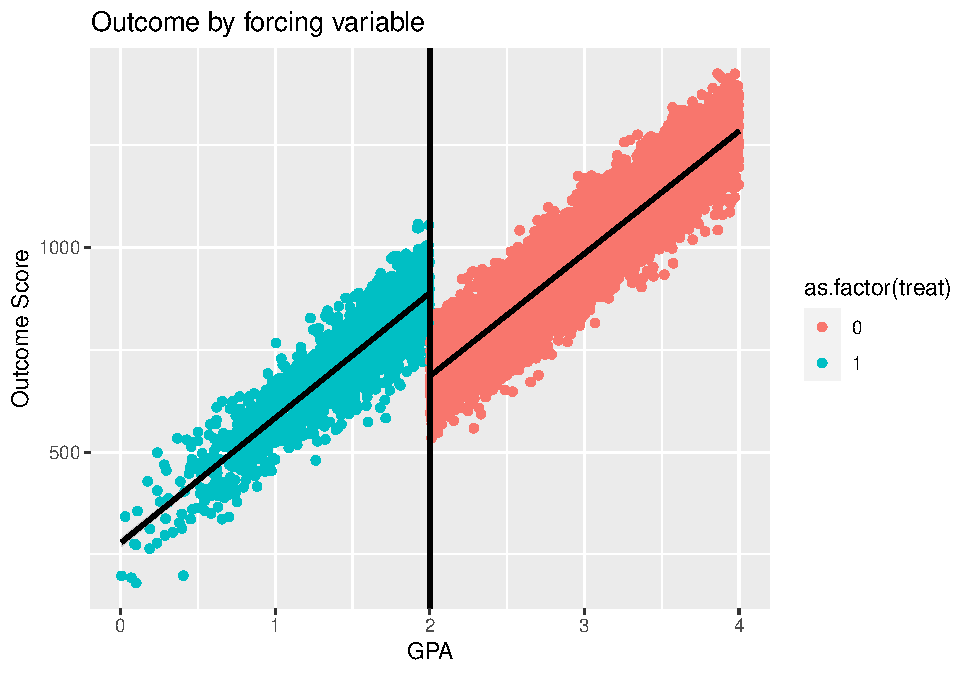
\includegraphics{EM2_PS4_Estrada_files/figure-latex/part1-1.pdf}

\subsection{1.2) Plot the density of the forcing
variable}\label{plot-the-density-of-the-forcing-variable}

You can also embed plots, for example:

\begin{Shaded}
\begin{Highlighting}[]
\NormalTok{plot2 <-}\StringTok{ }\KeywordTok{ggplot}\NormalTok{(data, }\KeywordTok{aes}\NormalTok{(gpa)) +}\StringTok{ }
\StringTok{  }\KeywordTok{geom_histogram}\NormalTok{(}\DataTypeTok{fill =} \StringTok{"blue"}\NormalTok{, }\DataTypeTok{color =} \StringTok{"lightblue"}\NormalTok{, }\DataTypeTok{binwidth =} \FloatTok{0.05}\NormalTok{) +}
\StringTok{  }\KeywordTok{labs}\NormalTok{(}\DataTypeTok{x =} \StringTok{"GPA"}\NormalTok{, }\DataTypeTok{y =} \StringTok{"Outcome Score"}\NormalTok{) +}\StringTok{ }\KeywordTok{ggtitle}\NormalTok{(}\StringTok{"Density by forcing variable"}\NormalTok{) +}
\StringTok{  }\KeywordTok{geom_vline}\NormalTok{(}\DataTypeTok{xintercept =} \NormalTok{gpa_cutoff, }\DataTypeTok{linewidth =} \DecValTok{1}\NormalTok{)}
\NormalTok{plot2}
\end{Highlighting}
\end{Shaded}

\begin{center}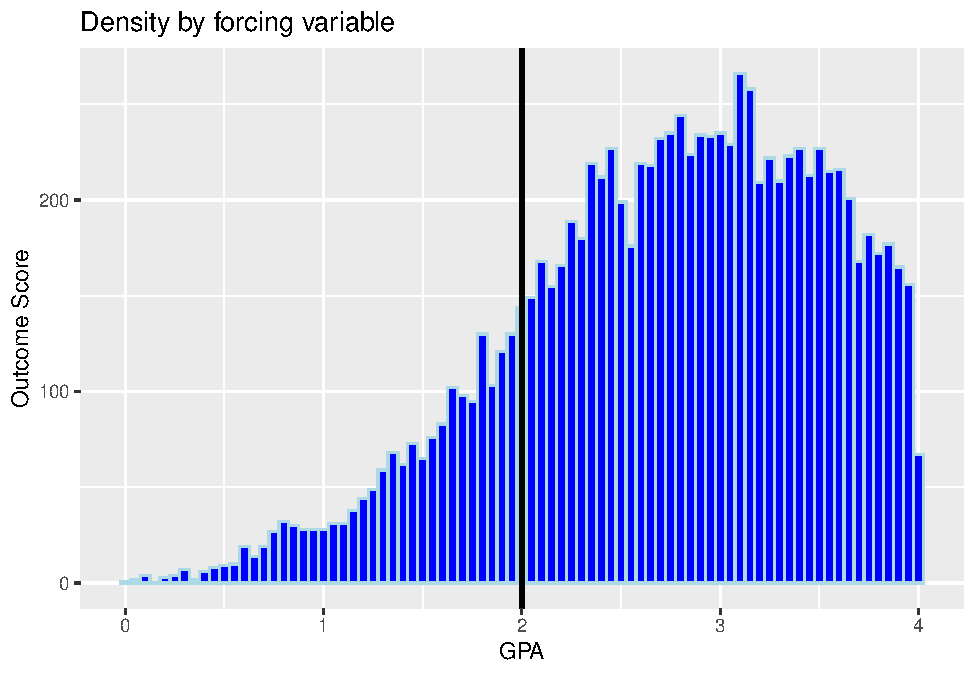
\includegraphics[width=0.75\linewidth]{EM2_PS4_Estrada_files/figure-latex/part2-1} \end{center}

\subsection{1.3) Estimate the effect using a local linear
regression}\label{estimate-the-effect-using-a-local-linear-regression}

\begin{Shaded}
\begin{Highlighting}[]
\NormalTok{reg3 =}\StringTok{ }\KeywordTok{lm}\NormalTok{(outcome_score ~}\StringTok{ }\NormalTok{treat +}\StringTok{ }\KeywordTok{I}\NormalTok{(gpa-gpa_cutoff) +}\StringTok{ }\KeywordTok{I}\NormalTok{(treat*(gpa-gpa_cutoff)) , }\DataTypeTok{data =} \NormalTok{data)}
\KeywordTok{stargazer}\NormalTok{(reg3, }\DataTypeTok{type =} \StringTok{"latex"}\NormalTok{, }\DataTypeTok{title =} \StringTok{"Local Linear Regression"}\NormalTok{, }\DataTypeTok{table.placement =} \StringTok{"H"}\NormalTok{,}
          \DataTypeTok{header=}\OtherTok{FALSE}\NormalTok{, }\DataTypeTok{no.space =} \NormalTok{T, }\DataTypeTok{omit.stat =} \StringTok{"f"}\NormalTok{)}
\end{Highlighting}
\end{Shaded}

\begin{table}[H] \centering 
  \caption{Local Linear Regression} 
  \label{} 
\begin{tabular}{@{\extracolsep{5pt}}lc} 
\\[-1.8ex]\hline 
\hline \\[-1.8ex] 
 & \multicolumn{1}{c}{\textit{Dependent variable:}} \\ 
\cline{2-2} 
\\[-1.8ex] & outcome\_score \\ 
\hline \\[-1.8ex] 
 treat & 203.537$^{***}$ \\ 
  & (2.780) \\ 
  I(gpa - gpa\_cutoff) & 299.659$^{***}$ \\ 
  & (1.281) \\ 
  I(treat \textasteriskcentered  (gpa - gpa\_cutoff)) & 6.113 \\ 
  & (3.812) \\ 
  Constant & 685.806$^{***}$ \\ 
  & (1.459) \\ 
 \hline \\[-1.8ex] 
Observations & 10,000 \\ 
R$^{2}$ & 0.896 \\ 
Adjusted R$^{2}$ & 0.896 \\ 
Residual Std. Error & 62.791 (df = 9996) \\ 
\hline 
\hline \\[-1.8ex] 
\textit{Note:}  & \multicolumn{1}{r}{$^{*}$p$<$0.1; $^{**}$p$<$0.05; $^{***}$p$<$0.01} \\ 
\end{tabular} 
\end{table}

\subsection{1.4) Estimate the effect using a local polynomial (of order
2 and 3)
regression}\label{estimate-the-effect-using-a-local-polynomial-of-order-2-and-3-regression}

\begin{Shaded}
\begin{Highlighting}[]
\NormalTok{reg41 =}\StringTok{ }\KeywordTok{lm}\NormalTok{(outcome_score ~}\StringTok{ }\NormalTok{treat +}\StringTok{ }\KeywordTok{I}\NormalTok{(gpa-gpa_cutoff) +}\StringTok{ }\KeywordTok{I}\NormalTok{(treat*(gpa-gpa_cutoff))+}
\StringTok{             }\KeywordTok{I}\NormalTok{((gpa-gpa_cutoff)^}\DecValTok{2}\NormalTok{) +}\StringTok{ }\KeywordTok{I}\NormalTok{(treat*(gpa-gpa_cutoff)^}\DecValTok{2}\NormalTok{), }\DataTypeTok{data =} \NormalTok{data)}
\CommentTok{#stargazer(reg41, type = "latex", title = "Estimate Effect Using Local Polynomial of Order 2", table.placement = "H", header=FALSE, no.space = T)}
\end{Highlighting}
\end{Shaded}

\begin{Shaded}
\begin{Highlighting}[]
\NormalTok{reg42 =}\StringTok{ }\KeywordTok{lm}\NormalTok{(outcome_score ~}\StringTok{ }\NormalTok{treat +}\StringTok{ }\KeywordTok{I}\NormalTok{(gpa-gpa_cutoff) +}\StringTok{ }\KeywordTok{I}\NormalTok{(treat*(gpa-gpa_cutoff))+}
\StringTok{             }\KeywordTok{I}\NormalTok{((gpa-gpa_cutoff)^}\DecValTok{2}\NormalTok{) +}\StringTok{ }\KeywordTok{I}\NormalTok{(treat*(gpa-gpa_cutoff)^}\DecValTok{2}\NormalTok{)+}
\StringTok{             }\KeywordTok{I}\NormalTok{((gpa-gpa_cutoff)^}\DecValTok{3}\NormalTok{) +}\StringTok{ }\KeywordTok{I}\NormalTok{(treat*(gpa-gpa_cutoff)^}\DecValTok{3}\NormalTok{), }\DataTypeTok{data =} \NormalTok{data)}
\KeywordTok{stargazer}\NormalTok{(reg3, reg41, reg42, }\DataTypeTok{type =} \StringTok{"latex"}\NormalTok{, }\DataTypeTok{title =} \StringTok{"Estimate Effect Using Local Polynomial of Order 2 and 3"}\NormalTok{,}
          \DataTypeTok{table.placement =} \StringTok{"H"}\NormalTok{, }\DataTypeTok{header=}\OtherTok{FALSE}\NormalTok{, }\DataTypeTok{no.space =} \NormalTok{T, }\DataTypeTok{omit.stat =} \StringTok{"f"}\NormalTok{)}
\end{Highlighting}
\end{Shaded}

\begin{table}[H] \centering 
  \caption{Estimate Effect Using Local Polynomial of Order 2 and 3} 
  \label{} 
\begin{tabular}{@{\extracolsep{5pt}}lccc} 
\\[-1.8ex]\hline 
\hline \\[-1.8ex] 
 & \multicolumn{3}{c}{\textit{Dependent variable:}} \\ 
\cline{2-4} 
\\[-1.8ex] & \multicolumn{3}{c}{outcome\_score} \\ 
\\[-1.8ex] & (1) & (2) & (3)\\ 
\hline \\[-1.8ex] 
 treat & 203.537$^{***}$ & 203.802$^{***}$ & 206.974$^{***}$ \\ 
  & (2.780) & (3.941) & (5.085) \\ 
  I(gpa - gpa\_cutoff) & 299.659$^{***}$ & 298.048$^{***}$ & 290.306$^{***}$ \\ 
  & (1.281) & (5.077) & (12.789) \\ 
  I(treat \textasteriskcentered  (gpa - gpa\_cutoff)) & 6.113 & 11.720 & 58.001$^{**}$ \\ 
  & (3.812) & (12.205) & (26.691) \\ 
  I((gpa - gpa\_cutoff)$\hat{\mkern6mu}$2) &  & 0.805 & 10.347 \\ 
  &  & (2.457) & (14.674) \\ 
  I(treat \textasteriskcentered  (gpa - gpa\_cutoff)$\hat{\mkern6mu}$2) &  & 2.012 & 55.470 \\ 
  &  & (7.800) & (37.519) \\ 
  I((gpa - gpa\_cutoff)$\hat{\mkern6mu}$3) &  &  & $-$3.181 \\ 
  &  &  & (4.823) \\ 
  I(treat \textasteriskcentered  (gpa - gpa\_cutoff)$\hat{\mkern6mu}$3) &  &  & 29.224$^{**}$ \\ 
  &  &  & (14.753) \\ 
  Constant & 685.806$^{***}$ & 686.375$^{***}$ & 687.755$^{***}$ \\ 
  & (1.459) & (2.268) & (3.086) \\ 
 \hline \\[-1.8ex] 
Observations & 10,000 & 10,000 & 10,000 \\ 
R$^{2}$ & 0.896 & 0.896 & 0.896 \\ 
Adjusted R$^{2}$ & 0.896 & 0.896 & 0.896 \\ 
Residual Std. Error & 62.791 (df = 9996) & 62.797 (df = 9994) & 62.791 (df = 9992) \\ 
\hline 
\hline \\[-1.8ex] 
\textit{Note:}  & \multicolumn{3}{r}{$^{*}$p$<$0.1; $^{**}$p$<$0.05; $^{***}$p$<$0.01} \\ 
\end{tabular} 
\end{table}

\end{document}
